%=================================================%
% Section:                        	              %
%    Results %
%=================================================%

\begin{center}
\section{Results}
\label{sec:Results}
\end{center}

%====================================================================%
% SubSection:                        	                             %
%    Results: Introduction %
%====================================================================%
\aboveSubSecSkip

\subsection{Introduction}
\label{sec:Results-Intro}

\noindent
	\indent This chapter contains TODO
				
\belowSubSecSkip

%====================================================================%
% SubSection:                        	                             %
%    Results: Multigroup Treatment %
%====================================================================%
\aboveSubSecSkip

\subsection{Multigroup Treatment}
\label{sec:Results-multigroup}

\noindent
	\indent This section evaluates the effectiveness of the multigroup treatment of the \gls{dmp}.  In order to verify the accuracy of the multigroup treatment, we compare predicted maximum principle violations to actual violations on the same problem benchmarked in \cite{WolLarDen}.  This problem is a one-dimensional Marshak wave, with a constant hot source on one side and an initially cold material. For a variety of time step sizes $\Delta_t$, several grid spacings $\Delta_x$ are selected and the first time step is solved and a check is performed for a maximum principle violation in the first cell, which is the limiting $\Delta_x$ and $\Delta_t$ for boundedness.  The smallest $\Delta_x$ which produces a maximum principle violation is noted.  The data set of these minimum violating $\Delta_x$ and corresponding $\Delta_t$ yields the bounding $\Delta_t$ and $\Delta_x$ set for this particular problem.

Parallel to the development of the \gls{dmp} bounds, each problem solution also predicts violations using the \gls{dmp} algorithm.  The predicted bounds are a set of minimum $\Delta_x$ that \emph{predict} a \gls{dmp} violation for each $\Delta_t$. The success of the \gls{dmp} algorithm is determined by how close the predicted violations match the actual violations.

In order to show the contrast between actual violations and predicted violations, a color and symbol scheme is used in Figure \ref{fig:results_multigroup}.  A ``plus'' mark denotes a successful prediction by the \gls{dmp} algorithm, while a failed prediction is indicated by a filled circle.  A red mark is an actual maximum principle violation, while a black mark is bounded.

\begin{figure}[htb]
\centering
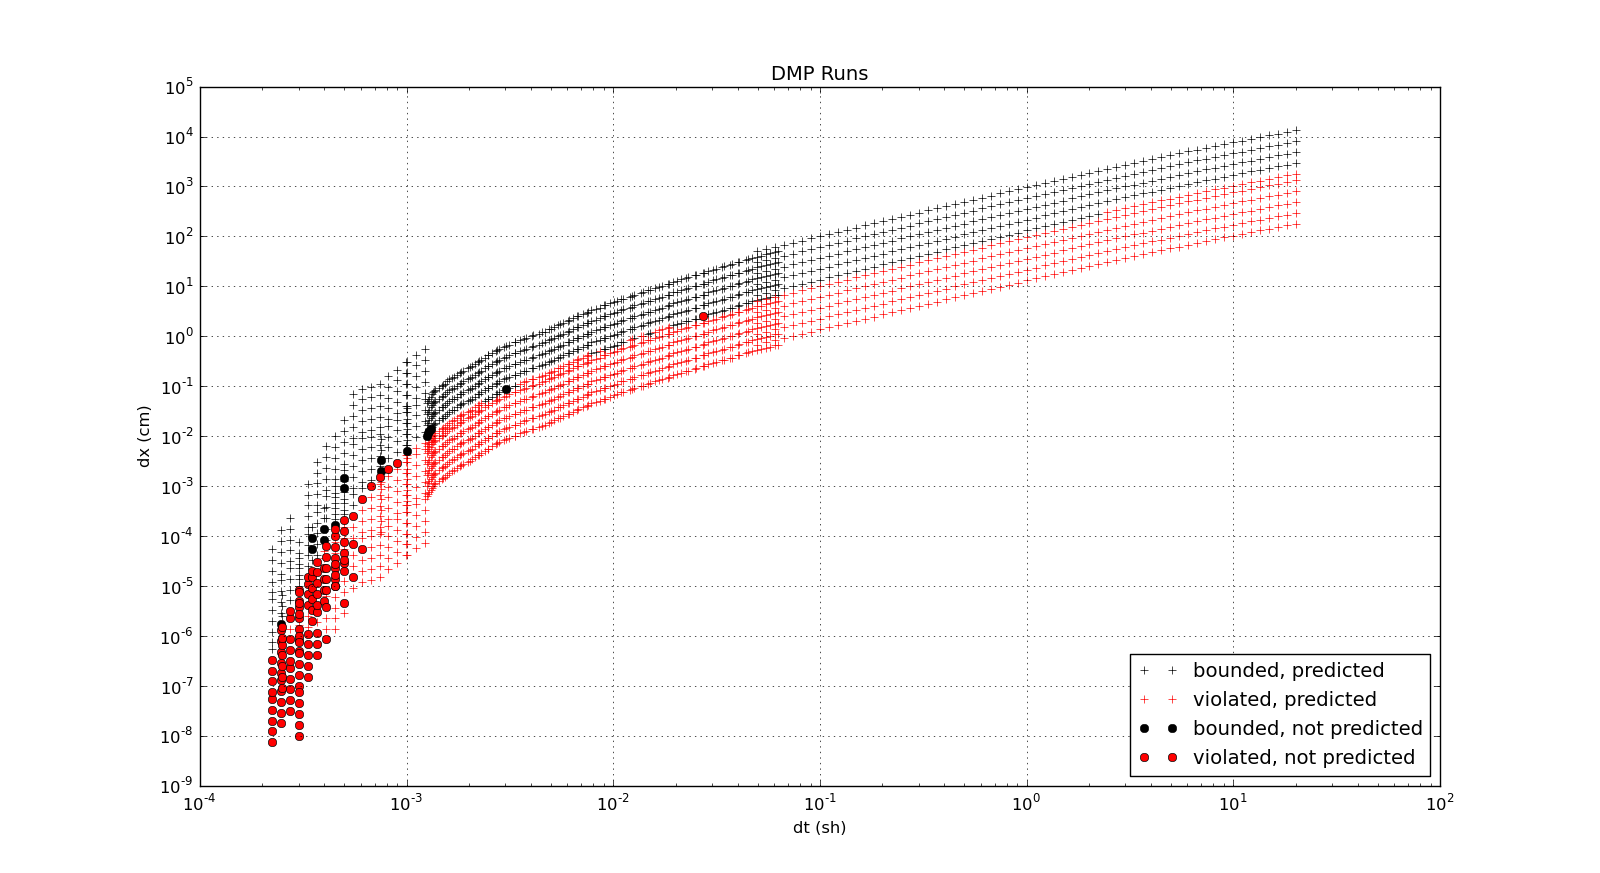
\includegraphics[width=\linewidth]{./graphics/mg_full}
\caption{Marshak Wave in One Dimension}
\label{fig:results_multigroup}
\end{figure}

For larger $\Delta_t$ and $\Delta_x$, the \gls{dmp} algorithm very accurately predicts maximum principle violations.  This accuracy diminishes with decreasing $\Delta_t$, however.  Recalling the truncation approximation made to the estimated energy deposited in a cell over a time step ($\tilde R$), the relative error introduced by the approximation increased significantly as $\Delta_t$ is less than about 0.001 shakes.  This leads us to expect a poorer performance by the \gls{dmp} as the time step nears $10^{-4}$ shakes, evident here.  To verify this failure of the \gls{dmp} algorithm is due to truncation terms, we test the pseudo-analytic \gls{dmp} from \cite{WolLarDen} and its truncation for several of the incorrect \gls{dmp} runs in Fig. \ref{fig:results_multigroup}.  If the pseudo-analytic \gls{dmp} with no truncation of $\tilde R$ correctly predicts maximum principle violations while the truncated \gls{dmp} does not, this provides strong suggestion that truncation is the leading effect in the \gls{dmp} poor performance for small $\Delta_x$.

TODO
				
\belowSubSecSkip

%====================================================================%
% SubSection:                        	                             %
%    Results: Non-Equilibrium Initial Conditions %
%====================================================================%
\aboveSubSecSkip

\subsection{Non-Equilibrium Conditions}
\label{sec:Results-noneq}

\noindent
	\indent In this section we explore non-equilibrium conditions where the radiation temperature and
material temperature are not equal at the beginning of a time step.  Physically this could occur when a small, thin material is bombarded by high-energy photons, where the temperature of the radiation field is substantially higher than the heat of the material for some time. TODO
				
\belowSubSecSkip

%====================================================================%
% SubSection:                        	                             %
%    Results: Multiple Dimensions %
%====================================================================%
\aboveSubSecSkip

\subsection{Multiple Sources}
\label{sec:Results-multiple}

\noindent
	\indent We now turn to considering a multidimensional case with hot sources on two neighboring sides of a material.  In particular, we address a problem with a choice of $\Delta_t$ and $\Delta_x$ such that neither surface source causes a maximum principle violation by itself, but when combined overheating occurs.  This tests the linear superposition assumption for estimated energy deposition.
\begin{figure}[htb]
\centering
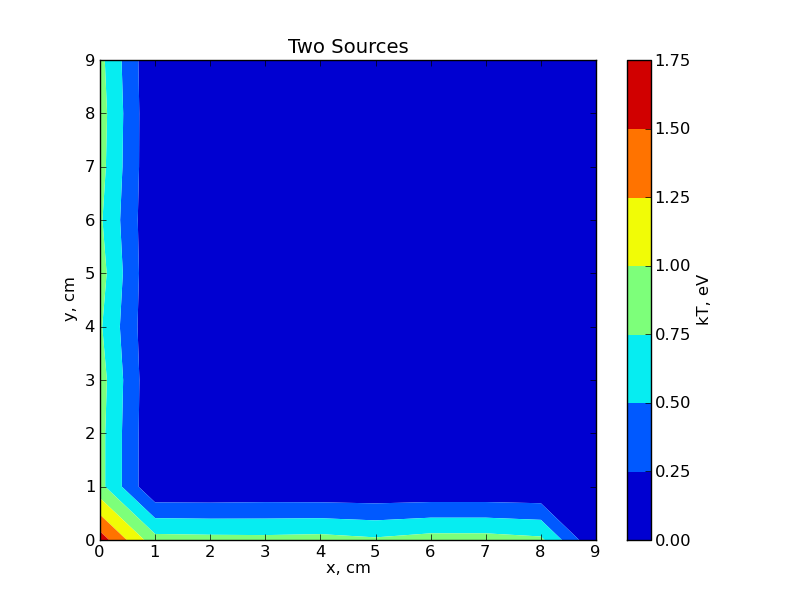
\includegraphics[width=\linewidth]{./graphics/2src}
\caption{Multiple Marshak Wave Sources}
\label{fig:results_2src}
\end{figure}
				
\belowSubSecSkip


%====================================================================%
% SubSection:                        	                             %
%    Results: Multiple Time Steps (aka T_u ~ T_0) %
%====================================================================%
\aboveSubSecSkip

\subsection{Small $\Delta T$}
\label{sec:Results-dT}

\noindent
	\indent An unexpected discovery about the characteristics of the \gls{dmp} emerged while observing multiple time steps as a Marshak wave distributes across the material.  The \gls{dmp} was used to predict violations on each cell of the mesh.  To avoid division-by-zero errors, if the estimated energy to be deposited in a cell $\tilde R$ is zero for all cells near the one being evaluated, the \gls{dmp} assumed no violations from that cell.  During the first time step, then, only the first cell is checked for \gls{dmp} violations for a 1D Marshak wave problem.  In successive steps, however, the \gls{dmp} incorrectly prediced maximum principle violations in cells where neighbor cell temperatures were very close to the cell's own temperature.  As it has been implemented to this point, this is a significant flaw in the implementation of the \gls{dmp} and deserves significant attention.  For now, we demonstrate the following using the grey case \gls{dmp} inequality to show how these false predictions come about.  

The grey, one-dimensional \gls{dmp} inequality is as follows: TODO reference earlier derivation
\begin{equation}\label{dT grey}
\Delta_t<\frac{c_v}{\sigma a c}\frac{1}{\frac{T_u^4-T_0^4}{T_u-T_0}\frac{1}{\Lambda}-4\alpha T_0^3}.
\end{equation}
We can represent a neighbor cell temperature $T_u$ that is higher than the local cell temperature $T_0$ as the cell temperature plus some difference in temperatures, or
\begin{equation}\label{dT}
T_u=T_0+\Delta T.
\end{equation}
Noting the fourth-order terms in Eq. \ref{dT grey}, we consider
\begin{equation}
T_u^4=T_0^4+4\Delta TT_0^3+6\Delta T^2T_0^2+4\Delta T^3T_0 + \Delta T^4,
\end{equation}
or, as $\Delta T\to0$, which is the case of interest here, 
\begin{equation}\label{dT trunc}
T_u^4=T_0^4+4\Delta TT_0^3+6\Delta T^2T_0^2+\mathcal{O}(\Delta T^3).
\end{equation}
Inserting Eqs. \ref{dT} and \ref{dT trunc} into Eq. \ref{dT grey},
\begin{equation}
\Delta_t<\frac{c_v}{\sigma a c}\frac{\Lambda}{4T_0^3(1-\Lambda\alpha)+6\Delta TT_0^3 + \mathcal{O}(\Delta T^2)}.
\end{equation}
If $\Lambda$ were strictly less than unity, this would not pose a problem; however, in many limiting cases TODO, $\Lambda>1$, which, for small $\Delta T$, reults in the \gls{dmp} requiring a negative time step in order to satisfy the inequality.  Rearranging, this leads to a litmus test for applying the \gls{dmp}; that is, if
\begin{equation}
\Delta T<=\frac{2}{3}(\Lambda\alpha-1)T_0,
\end{equation}
the \gls{dmp} will be an inaccurate predictor of maxium principle violations.  Fortunately, since this limit is only of concern when $\Delta T$ is small, and overheating only occurs when $\Delta T$ is large, this test should restore accuracy to the \gls{dmp} algorithm.  A similar result for the multifrequency case is a desirable pursuit for the future. \\
TODO move this derivation into the methods section\\
In Figs. \ref{fig:results_multistep1} and \ref{fig:results_multistep2}, the benefit of the switch is demonstrated.  Black dots indicate a maximum principle violation prediction, and black crosses show where the \gls{dmp} predicts no violation.

\begin{figure}[H]
\centering
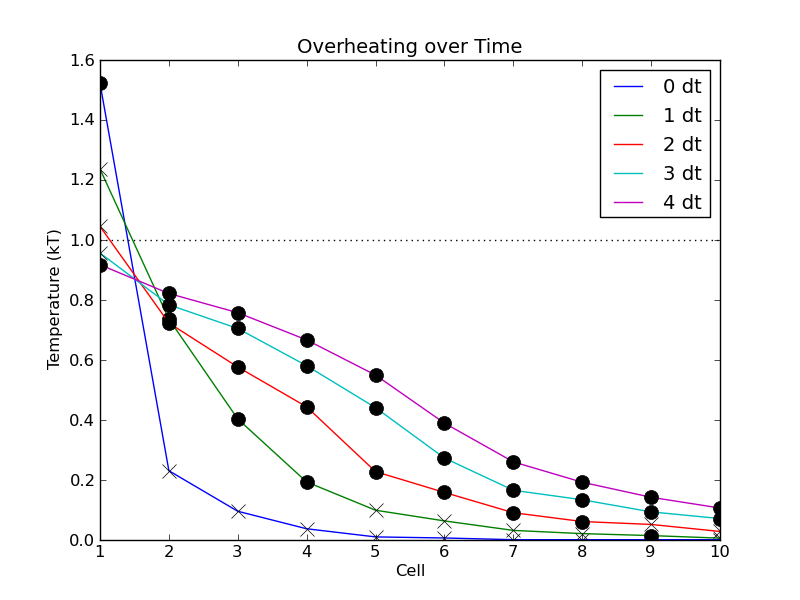
\includegraphics[width=0.7\linewidth]{./graphics/multistep1}
\caption{Multiple Time Steps, Before Switch}
\label{fig:results_multistep1}
\end{figure}
\begin{figure}[H]
\centering
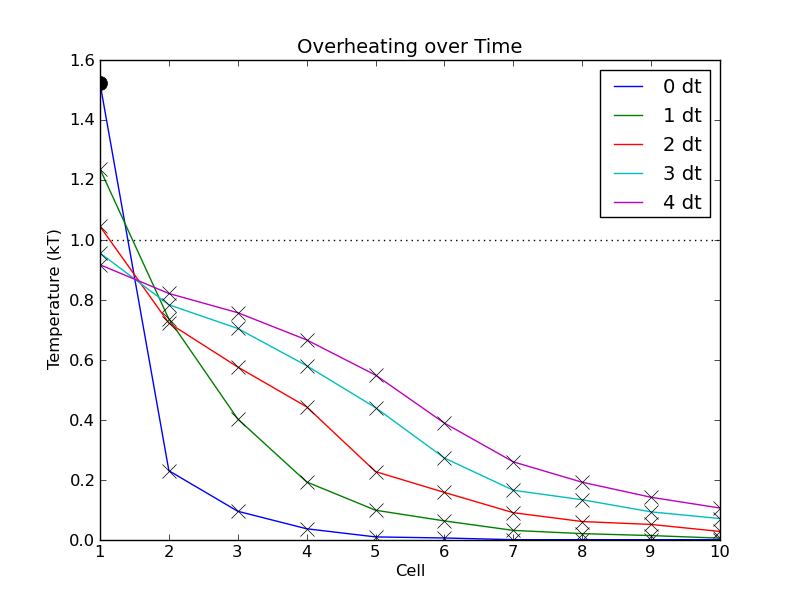
\includegraphics[width=0.7\linewidth]{./graphics/multistep2}
\caption{Multiple Time Steps, After Switch}
\label{fig:results_multistep2}
\end{figure}
\belowSubSecSkip

%=====================================================================%
% SubSection:                        	                              %
%     Results: Summary %
%=====================================================================%
\subsection{Summary}
\label{sec:Results-Summary}

\noindent
	\indent TODO










